\documentclass[hyperref={bookmarks=false},aspectratio=169]{beamer}
\usepackage[utf8]{inputenc}
\usepackage{standalone}
% ---------------  Define theme and color scheme  -----------------
\usetheme[sidebarleft]{CEIT}  % 3 options: minimal, sidebarleft, sidebarright

%\setbeamertemplate{footline}[frame number]

% ------------  Information on the title page  --------------------
\title[CEIT]
{\bfseries{Centre of Excellence in IT}}

\subtitle{Courses}

\author[Jishnu T U] %\& Managed]
{Jishnu T U\inst{1} } %\and Managed\inst{2}}

\institute[CEIT]
{
  \inst{1}
  Trainer\\
  Centre of Excellence in IT,PNG
 % \and
 % \inst{2}
 % Trainer\\
 % Centre of Excellence in IT,PNG
}

\date[CEIT, 2014]
{Centre of Excellence in IT,PNG October 2019}
%------------------------------------------------------------

%------------------------------------------------------------
%The next block of commands puts the table of contents at the 
%beginning of each section and highlights the current section:

\AtBeginSection[]
{
  \begin{frame}
    \frametitle{Table of Contents}
    \tableofcontents[currentsection]
  \end{frame}
}

%------------------------------------------------------------


\begin{document}

\frame{\titlepage}  % Creates title page

%---------   table of contents after title page  ------------
\begin{frame}
\frametitle{Table of Contents}
\tableofcontents
\end{frame}
%---------------------------------------------------------

\section{first topic}

%---------------------------------------------------------
%Changing visivility of the text
\begin{frame}
\frametitle{frame title 1}
Every Halloween, Dabney House conducts the infamous ``Millikan pumpkin-drop experiment'' from the top of Millikan Library, the highest point on campus.

\begin{itemize}
    \item<1-> A claim was once made that the shattering of a pumpkin frozen in liquid nitrogen and dropped from a sufficient height would produce a triboluminescent spark. 
    \item<2-> This yearly event involves a crowd of observers, who try to spot the elusive spark.
    \item<3-> The title of the event is an oblique reference to the famous Millikan oil-drop experiment which measured $e$, the elemental unit of electrical charge.
\end{itemize}

\end{frame}
\section{Internet of Things}
\begin{frame}
	\frametitle{Certificate Course in Internet of Things}
	\begin{columns}
		
	\column{0.45\textwidth}
			
		\begin{figure}
			
\includegraphics[width=200pt,height=150pt]{figures/course_iot.jpg}
		\end{figure}
	
	\column{0.55\textwidth}

	\begin{block}{Description}
	
		\begin{enumerate}
			\item Embedded	Linux to develop for IoT. 
			\item Wireless Network \& Communication protocols.
			\item IoT prototyping using NodeJS and Python for development.
			\item Cloud Platforms for IoT.
		\end{enumerate}
	  	  
	\end{block}

	\end{columns}
\end{frame}








\section{Web Development}
\begin{frame}
	\frametitle{Certificate Course in Java Programming}
	\begin{columns}
		\column{0.45\textwidth}
	
	\begin{figure}
		
\includegraphics[width=180pt,height=150pt]{figures/course_jp.jpg}
	\end{figure}
	
	\column{0.55\textwidth}
	
	\begin{block}{Description}
		
		\begin{enumerate}
			\item Core Java and Advanced Java programming. 
			\item Database Technologies.
			\item Foundations of Web Technologies.
			\item Enterprise Java for Servlets, Java Server Pages.
		\end{enumerate}
		
	\end{block}
	
\end{columns}
\end{frame}

\begin{frame}
	\frametitle{Certificate Course in MS.Net}
	\begin{columns}
		\column{0.45\textwidth}
	
	\begin{figure}
		
\includegraphics[width=200pt,height=150pt]{figures/course_msnet.jpg}
	\end{figure}
	
	\column{0.55\textwidth}
	
	\begin{block}{Description}
		
		\begin{enumerate}
			\item MS .NET 4.5 Framework using C\#.
			\item Database Technologies.
			\item Foundations of Web Technologies.
			\item MS .Net Window programming.
			\item MS .Net Web based programming.
		\end{enumerate}
		
	\end{block}
	
\end{columns}
\end{frame}

\begin{frame}
	\frametitle{Certificate Course in Advanced Web Technology}
	\begin{columns}
		\column{0.45\textwidth}
	
	\begin{figure}
		
\includegraphics[width=200pt,height=150pt]{figures/course_awt.jpg}
	\end{figure}
	
	\column{0.55\textwidth}
	
	\begin{block}{Description}
		
		\begin{enumerate}
			\item Web Programming – I (HTML, CSS, Ajax). 
			\item Web Programming – II (PHP, Java scripts).
			\item Database Concepts.
			\item Internet Terminologies
		\end{enumerate}
		
	\end{block}
	
\end{columns}
\end{frame}

\begin{frame}
	\frametitle{ {\large Certificate Course in Multimedia Website Designing}}
	\begin{columns}
		\column{0.45\textwidth}
	
	\begin{figure}
		
\includegraphics[width=200pt,height=150pt]{figures/course_mwd.jpg}
	\end{figure}
	
	\column{0.55\textwidth}
	
	\begin{block}{Description}
		
		\begin{enumerate}
			\item HTML Scripting. 
			\item Javascript,CSS,JQuery.
			\item Interactive Flash Animation
		\end{enumerate}
		
	\end{block}
	
\end{columns}
\end{frame}
\section{Mobile Applications}
\begin{frame}
	\frametitle{Certificate Course in Android Programming}
		\begin{columns}
		
		\column{0.45\textwidth}
		
		\begin{figure}
			
\includegraphics[width=200pt,height=150pt]{figures/course_ap.jpg}
		\end{figure}
		
		\column{0.55\textwidth}
		
		\begin{block}{Description}
			
			\begin{enumerate}
				\item Java Programming. 
				\item Mobile and Wireless Technologies.
				\item Android Programming.
				\item Database Concepts.
			\end{enumerate}
			
		\end{block}
		
	\end{columns}
\end{frame}
\section{Big Data}
\begin{frame}
	\frametitle{Certificate Course in Big Data Technologies}
\end{frame}

\begin{frame}
	\frametitle{Certificate Course in Big Data Analytics}
\end{frame}
\section{Database Administration}
\begin{frame}
	\frametitle{Certificate Course in Database Management }
\end{frame}
\section{Infrastructure and Network Security}
\begin{frame}
	\frametitle{Certificate Course in Network Security}
\end{frame}
\begin{frame}
	\frametitle{{\large Certificate Course in Ethical Hacking \& Information Security}}
\end{frame}
\section{System Administration and Networking}
\begin{frame}
	\frametitle{{\large Certificate Course in Linux System Administration}}
		\begin{columns}
		
		\column{0.45\textwidth}
		
		\begin{figure}
			
\includegraphics[width=180pt,height=150pt]{figures/course_lsa.jpg}
		\end{figure}
		
		\column{0.55\textwidth}
		
		\begin{block}{Description}
			
			\begin{enumerate}
				\item Fundamentals of Networking. 
				\item Linux Administration.
				\item System Administration.
			\end{enumerate}
			
		\end{block}
		
	\end{columns}
\end{frame}

\begin{frame}
	\frametitle{Certificate Course in Network Administration}
		\begin{columns}
		
		\column{0.45\textwidth}
		
		\begin{figure}
			
\includegraphics[width=180pt,height=150pt]{figures/course_na.jpg}
		\end{figure}
		
		\column{0.55\textwidth}
		
		\begin{block}{Description}
			
			\begin{enumerate}
				\item Computer Networking. 
				\item Network Administration.
				\item Network Defense and Countermeasures.
			\end{enumerate}
			
		\end{block}
		
	\end{columns}
\end{frame}

\begin{frame}
	\frametitle{{\large Certificate Course in Data Communication and Networking}}
		\begin{columns}
		
		\column{0.45\textwidth}
		
		\begin{figure}
			
\includegraphics[width=180pt,height=150pt]{figures/course_dcn.jpg}
		\end{figure}
		
		\column{0.55\textwidth}
		
		\begin{block}{Description}
			
			\begin{enumerate}
				\item Introduction to Networking. 
				\item Windows Server 2016.
				\item Linux OS administration and configuration.
			\end{enumerate}
			
		\end{block}
		
	\end{columns}
\end{frame}
\section{IT Applications} 
\begin{frame}
	\frametitle{Certificate Course in Software Testing}
		\begin{columns}
		
		\column{0.45\textwidth}
		
		\begin{figure}
			
\includegraphics[width=200pt,height=150pt]{figures/course_st.jpg}
		\end{figure}
		
		\column{0.55\textwidth}
		
		\begin{block}{Description}
			
			\begin{enumerate}
				\item Software Development Life Cycle. 
				\item Software Testing – Manual.
				\item Software Testing – Automation.
			\end{enumerate}
			
		\end{block}
		
	\end{columns}
\end{frame}
\begin{frame}
	\frametitle{Certificate Course in Office Automation}
		\begin{columns}
		
		\column{0.45\textwidth}
		
		\begin{figure}
			
\includegraphics[width=200pt,height=150pt]{figures/course_oa.jpg}
		\end{figure}
		
		\column{0.55\textwidth}
		
		\begin{block}{Description}
			
			\begin{enumerate}
				\item Client Operating System (Windows 10, Ubuntu). 
				\item MS Office 2016
				\item Database Concepts
				\item Database Management using MS access
			\end{enumerate}
			
		\end{block}
		
	\end{columns}
\end{frame}
\begin{frame}
	\frametitle{Certificate Course in Information Technology}
		\begin{columns}
		
		\column{0.45\textwidth}
		
		\begin{figure}
			
\includegraphics[width=200pt,height=150pt]{figures/course_it.jpg}
		\end{figure}
		
		\column{0.55\textwidth}
		
		\begin{block}{Description}
			
			\begin{enumerate}
				\item Office Automation Tools. 
				\item Computer Fundamentals.
				\item Communication using PC.
				\item Overview of Networking.
				\item Database Concepts and MS Access.
			\end{enumerate}
			
		\end{block}
		
	\end{columns}
\end{frame}

%\begin{frame}
\frametitle{Frame Title 2}
\begin{figure}
    \centering
    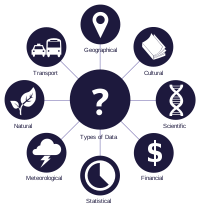
\includegraphics[width=400pt,height=210pt]{figures/fig1.png}
    \caption{``Hollywood is still mad about that, author of \emph{Legends of tech III: Techer In the Dark.}}
    \label{fig:hollywood}
\end{figure}

\end{frame}
%---------------------------------------------------------
%\section{Internet of Things}
\begin{frame}
	\frametitle{Certificate Course in Internet of Things}
	\begin{columns}
		
	\column{0.45\textwidth}
			
		\begin{figure}
			
\includegraphics[width=200pt,height=150pt]{figures/course_iot.jpg}
		\end{figure}
	
	\column{0.55\textwidth}

	\begin{block}{Description}
	
		\begin{enumerate}
			\item Embedded	Linux to develop for IoT. 
			\item Wireless Network \& Communication protocols.
			\item IoT prototyping using NodeJS and Python for development.
			\item Cloud Platforms for IoT.
		\end{enumerate}
	  	  
	\end{block}

	\end{columns}
\end{frame}








%---------------------------------------------------------

%%Two columns
\begin{frame}
\frametitle{Frame Title 4}

\begin{columns}

\column{0.45\textwidth}

\begin{figure}
    \centering
    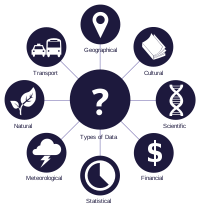
\includegraphics[scale=.4]{figures/fig1.png}
    \caption{``Hollywood is still mad about that, author of \emph{Legends of tech III: Techer In the Dark.}}
    \label{fig:hollywood_prank}
\end{figure}


\column{0.55\textwidth}
In May 1987, undergraduates from Page and Ricketts houses combined forces (and several hundred dollars) to purchase enough black and white plastic, transformed the Hollywood sign to read ``Caltech''.

\small{(Reference: http://www.admissions.caltech.edu/pranks)}

\end{columns}
\end{frame}
%---------------------------------------------------------

%---------------------------------------------------------


\end{document}